\documentclass[tikz, border=0pt, 12pt, convert,
convert={
	outext=.svg,
	command=\unexpanded{
			pdf2svg \infile\space \outfile\space all
			&& pdftocairo -r 300 -png \infile\space
		}
}]{standalone}
\usepackage{xeCJK}
% \setCJKmainfont{Source Han Serif TC}
\setCJKmainfont{Source Han Sans TC}
\setCJKsansfont{Source Han Sans TC}

\usepackage{scalefnt}
\usepackage{lmodern}
\usepackage{tikz}
\usepackage{graphicx}
\usetikzlibrary{shapes.geometric, arrows, positioning, calc, arrows.meta}

\tikzstyle{startstop} = [rectangle, rounded corners, minimum width=3cm, minimum height=1cm,text centered,  text=white, draw=black, fill=colorStarstop]

% process
\tikzstyle{process} = [rectangle, minimum width=3cm, minimum height=1cm, text centered, text=white, draw=black, fill=colorPro]

% decision
\tikzstyle{decision}=[diamond, minimum width=3cm, minimum height=1cm, text centered, draw=black , fill=colorDec]

\usetikzlibrary{positioning}

\tikzset{
	subprocess/.style = {rectangle, draw=black, semithick, fill=orange!30,
		minimum width=#1, minimum height=1cm, inner xsep=3mm, % <-- changed
		text width =\pgfkeysvalueof{/pgf/minimum width}-2*\pgfkeysvalueof{/pgf/inner xsep},
		align=flush center,
		path picture={\draw
			([xshift =2mm] \ppbb.north west) -- ([xshift= 2mm] \ppbb.south west)
			([xshift=-2mm] \ppbb.north east) -- ([xshift=-2mm] \ppbb.south east);
		},
	},
	subprocess/.default = 24mm % <-- added
}% end of tikzset

% comment
\tikzstyle{comment}=[dashed, draw=black, fill=gray!10, minimum width=3cm, minimum height=1cm, text centered]

\tikzstyle{docstring}=[draw=orange, fill=white, minimum width=50mm, text width=80mm, minimum height=1cm]

% arrows
\tikzstyle{arrow} = [ultra thick,->,>=stealth, line width=1.5mm]
\tikzstyle{arrow_med} = [thick,->,>=stealth, line width=1mm]

% comment
\tikzstyle{comment}=[dashed, draw=black, fill=gray!10, minimum width=3cm, minimum height=1cm, text centered]

\tikzstyle{docstring}=[draw=orange, fill=white, minimum width=50mm, text width=80mm, minimum height=1cm]

% arrows
\tikzstyle{arrow} = [ultra thick,->,>=stealth, line width=1.5mm]

\definecolor{colorStarstop}{RGB}{174, 23, 21}
\definecolor{colorPro}{RGB}{0, 175, 121}
\definecolor{colorDec}{RGB}{255, 192, 0}
\definecolor{colorYes}{RGB}{51, 153, 51}
\definecolor{colorNo}{RGB}{255, 0, 0}
\definecolor{forestGreen}{RGB}{44, 180, 44}
\definecolor{paleBlue}{RGB}{102, 153, 255}

\begin{document}

	\scalefont{1.0}

	% \begin{tikzpicture}[font=\ttfamily\bfseries, baseline=(current bounding box.north), scale=1.0, every node/.style={scale=1}]
\begin{tikzpicture}[baseline=(current bounding box.north), scale=1.0, every node/.style={scale=1}]

	\matrix[column sep=20mm, row sep=10mm]
	{
		% start
		&
		&
		& \node (start)[startstop]{开始};
		& \\

		% round to nearest, tie to even
		&
		&
		& \node (pBankersRound)[process, text width=50mm]{四舍六入五留双 \\ (亦称作“银行家数值修约”)};
		& \node (cBankersRound)[comment, text width=60mm]{\textcolor{red}{不要使用Python自带的“round()”函数。应使用“decimal”模块。}};
		& \\

		% round to nearest, tie to even
		&
		&
		& \node (pRound2Nth)[process, text width=40mm]{保留$n$位数字};
		& \node (expRound2Nth)[comment, text width=60mm]{例:保留两位数字};
		& \\

		&
		& \node (pNoRound)[process, text width=40mm]{不需要修约};
		& \node (decNP1Zero)[decision, text width=30mm]{第$n+1$位数字为零或不存在?};
		& \\

		% n+1 th
		&
		& \node (pRoundDown)[process, text width=40mm]{舍位};
		& \node (decNP1)[decision, text width=25mm]{第$n+1$位数字是?};
		& \node (pRoundUp)[process, text width=40mm]{进位};
		& \\

		% n+2 th
		&
		&
		& \node (decNP2)[decision, text width=25mm]{第$n+2$位数字是?};
		& \\

		&
		&
		& \node (decNP1_2)[decision, text width=30mm]{第$n$位数字是奇或偶?};
		& \\

		% end
		&
		&
		& \node (end)[startstop]{结束};
		& \\
	};

	\node(expNoRound)[comment, yshift=25mm, text width=40mm] at (pNoRound){例:\\ $1.250 \Rightarrow 0$ \\ 结果 $= 1.25$};

	\node(expRoundDownNP1)[comment, yshift=27mm, text width=40mm] at (pRoundDown) {例:\\ $1.254 \Rightarrow 4$ \\ 结果 $= 1.25$};

	\node(expRoundUpNP1)[comment, yshift=27mm, text width=40mm] at (pRoundUp) {例:\\ $1.256 \Rightarrow 6$ \\ 结果 $= 1.26$};

	\node(expNP2)[comment, xshift=47mm, yshift=25mm, text width=50mm] at (decNP2) {例:\\ $1.2551 \Rightarrow 1, 结果 = 1.26$ \\ $1.2651 \Rightarrow 1, 结果 = 1.27$};

	\node(expNP1_2_odd)[comment, xshift=45mm, yshift=19mm, text width=40mm] at (decNP1_2) {例:\\ $1.2550 \Rightarrow 5$\ \textcolor{colorNo}{(奇)} \\ 结果 $= 1.26$};
	\node(expNP1_2_even)[comment, xshift=-43mm, yshift=19mm, text width=40mm] at (decNP1_2) {例:\\ $1.2650 \Rightarrow 6$\ \textcolor{colorYes}{(偶)} \\ 结果 $= 1.26$};

	% lines and arrows
	\draw[arrow](start) -- (pBankersRound);
	\draw[arrow](pBankersRound) -- (pRound2Nth);
	\draw[arrow](pRound2Nth) -- (decNP1Zero);
	\draw[arrow, , color=colorNo](decNP1Zero)node[anchor=north,	xshift=5mm, yshift=-20mm]{否} -- (decNP1);

	% 拐弯用
	\coordinate[left of=pRoundDown, xshift=-20mm] (dummy1);
	\coordinate[right of=pRoundUp, xshift=20mm] (dummy2);

	\draw[arrow, , color=colorYes](decNP1Zero)node[anchor=east, xshift=-25mm, yshift=5mm]{是} -- (pNoRound);

	\draw[arrow](pNoRound) -| (dummy1) |- (end);

	\draw[arrow, color=colorYes](decNP1)node[anchor=south, xshift=-32mm, yshift=1mm]{小于等于4} -- (pRoundDown);
	\draw[arrow, color=colorNo](decNP1)node[anchor=south, xshift=34mm, yshift=1mm]{大于等于6} -- (pRoundUp);
	\draw[arrow](decNP1)node[anchor=north, xshift=10mm, yshift=-20mm]{等于5} -- (decNP2);

	\draw[arrow, color=colorNo](decNP2)node[anchor=south, xshift=32mm, yshift=1mm]{大于等于1} -| (pRoundUp);
	\draw[arrow](decNP2)node[anchor=north, xshift=12mm, yshift=-19mm]{为零或无} -- (decNP1_2);

	\draw[arrow, color=colorNo](decNP1_2)node[anchor=south, xshift=32mm, yshift=1mm]{奇} -| (pRoundUp);
	\draw[arrow, color=colorYes](decNP1_2)node[anchor=south, xshift=-32mm, yshift=1mm]{偶} -| (pRoundDown);

	\draw[arrow](pRoundDown) -- (dummy1) |- (end);
	\draw[arrow](pRoundUp) -- (dummy2) |- (end);

	% dashed line
	\draw[dashed] (cBankersRound) -- (pBankersRound);
	\draw[dashed] (expRound2Nth) -- (pRound2Nth);
	\draw[dashed] (expNoRound) -- (decNP1Zero);
	\draw[dashed] (expRoundDownNP1) -- (decNP1);
	\draw[dashed] (expRoundUpNP1) -- (decNP1);
	\draw[dashed] (expNP2) -- (decNP2);
	\draw[dashed] (expNP1_2_odd) -- (decNP1_2);
	\draw[dashed] (expNP1_2_even) -- (decNP1_2);

\end{tikzpicture}
	% \begin{tikzpicture}[font=\ttfamily\bfseries, baseline=(current bounding box.north), scale=1.0, every node/.style={scale=1}]
\begin{tikzpicture}[baseline=(current bounding box.north), scale=1.0, every node/.style={scale=1}]

	\matrix[column sep=20mm, row sep=10mm]
	{
		% start
		&
		&
		& \node (start)[startstop]{開始};
		& \\

		% round to nearest, tie to even
		&
		&
		& \node (pBankersRound)[process, text width=50mm]{四捨六入五留雙 \\ (亦稱作“銀行家數值修約”)};
		& \node (cBankersRound)[comment, text width=60mm]{\textcolor{red}{不要使用Python自帶的“round()”函數。應使用“decimal”模塊。}};
		& \\

		% round to nearest, tie to even
		&
		&
		& \node (pRound2Nth)[process, text width=40mm]{保留$n$位數字};
		& \node (expRound2Nth)[comment, text width=60mm]{例:保留兩位數字};
		& \\

		&
		& \node (pNoRound)[process, text width=40mm]{不需要修約};
		& \node (decNP1Zero)[decision, text width=30mm]{第$n+1$位數字爲零或不存在?};
		& \\

		% n+1 th
		&
		& \node (pRoundDown)[process, text width=40mm]{舍位};
		& \node (decNP1)[decision, text width=25mm]{第$n+1$位數字是?};
		& \node (pRoundUp)[process, text width=40mm]{進位};
		& \\

		% n+2 th
		&
		&
		& \node (decNP2)[decision, text width=25mm]{第$n+2$位數字是?};
		& \\

		&
		&
		& \node (decNP1_2)[decision, text width=30mm]{第$n$位數字是奇或偶?};
		& \\

		% end
		&
		&
		& \node (end)[startstop]{結束};
		& \\
	};

	\node(expNoRound)[comment, yshift=25mm, text width=40mm] at (pNoRound){例:\\ $1.250 \Rightarrow 0$ \\ 結果 $= 1.25$};

	\node(expRoundDownNP1)[comment, yshift=27mm, text width=40mm] at (pRoundDown) {例:\\ $1.254 \Rightarrow 4$ \\ 結果 $= 1.25$};

	\node(expRoundUpNP1)[comment, yshift=27mm, text width=40mm] at (pRoundUp) {例:\\ $1.256 \Rightarrow 6$ \\ 結果 $= 1.26$};

	\node(expNP2)[comment, xshift=47mm, yshift=25mm, text width=50mm] at (decNP2) {例:\\ $1.2551 \Rightarrow 1, 結果 = 1.26$ \\ $1.2651 \Rightarrow 1, 結果 = 1.27$};

	\node(expNP1_2_odd)[comment, xshift=45mm, yshift=19mm, text width=40mm] at (decNP1_2) {例:\\ $1.2550 \Rightarrow 5$\ \textcolor{colorNo}{(奇)} \\ 結果 $= 1.26$};
	\node(expNP1_2_even)[comment, xshift=-43mm, yshift=19mm, text width=40mm] at (decNP1_2) {例:\\ $1.2650 \Rightarrow 6$\ \textcolor{colorYes}{(偶)} \\ 結果 $= 1.26$};

	% lines and arrows
	\draw[arrow](start) -- (pBankersRound);
	\draw[arrow](pBankersRound) -- (pRound2Nth);
	\draw[arrow](pRound2Nth) -- (decNP1Zero);
	\draw[arrow, , color=colorNo](decNP1Zero)node[anchor=north,	xshift=5mm, yshift=-20mm]{否} -- (decNP1);

	% 拐弯用
	\coordinate[left of=pRoundDown, xshift=-20mm] (dummy1);
	\coordinate[right of=pRoundUp, xshift=20mm] (dummy2);

	\draw[arrow, , color=colorYes](decNP1Zero)node[anchor=east, xshift=-25mm, yshift=5mm]{是} -- (pNoRound);

	\draw[arrow](pNoRound) -| (dummy1) |- (end);

	\draw[arrow, color=colorYes](decNP1)node[anchor=south, xshift=-32mm, yshift=1mm]{小於等於4} -- (pRoundDown);
	\draw[arrow, color=colorNo](decNP1)node[anchor=south, xshift=34mm, yshift=1mm]{大於等於6} -- (pRoundUp);
	\draw[arrow](decNP1)node[anchor=north, xshift=10mm, yshift=-20mm]{等於5} -- (decNP2);

	\draw[arrow, color=colorNo](decNP2)node[anchor=south, xshift=32mm, yshift=1mm]{大於等於1} -| (pRoundUp);
	\draw[arrow](decNP2)node[anchor=north, xshift=12mm, yshift=-19mm]{爲零或無} -- (decNP1_2);

	\draw[arrow, color=colorNo](decNP1_2)node[anchor=south, xshift=32mm, yshift=1mm]{奇} -| (pRoundUp);
	\draw[arrow, color=colorYes](decNP1_2)node[anchor=south, xshift=-32mm, yshift=1mm]{偶} -| (pRoundDown);

	\draw[arrow](pRoundDown) -- (dummy1) |- (end);
	\draw[arrow](pRoundUp) -- (dummy2) |- (end);

	% dashed line
	\draw[dashed] (cBankersRound) -- (pBankersRound);
	\draw[dashed] (expRound2Nth) -- (pRound2Nth);
	\draw[dashed] (expNoRound) -- (decNP1Zero);
	\draw[dashed] (expRoundDownNP1) -- (decNP1);
	\draw[dashed] (expRoundUpNP1) -- (decNP1);
	\draw[dashed] (expNP2) -- (decNP2);
	\draw[dashed] (expNP1_2_odd) -- (decNP1_2);
	\draw[dashed] (expNP1_2_even) -- (decNP1_2);

\end{tikzpicture}
	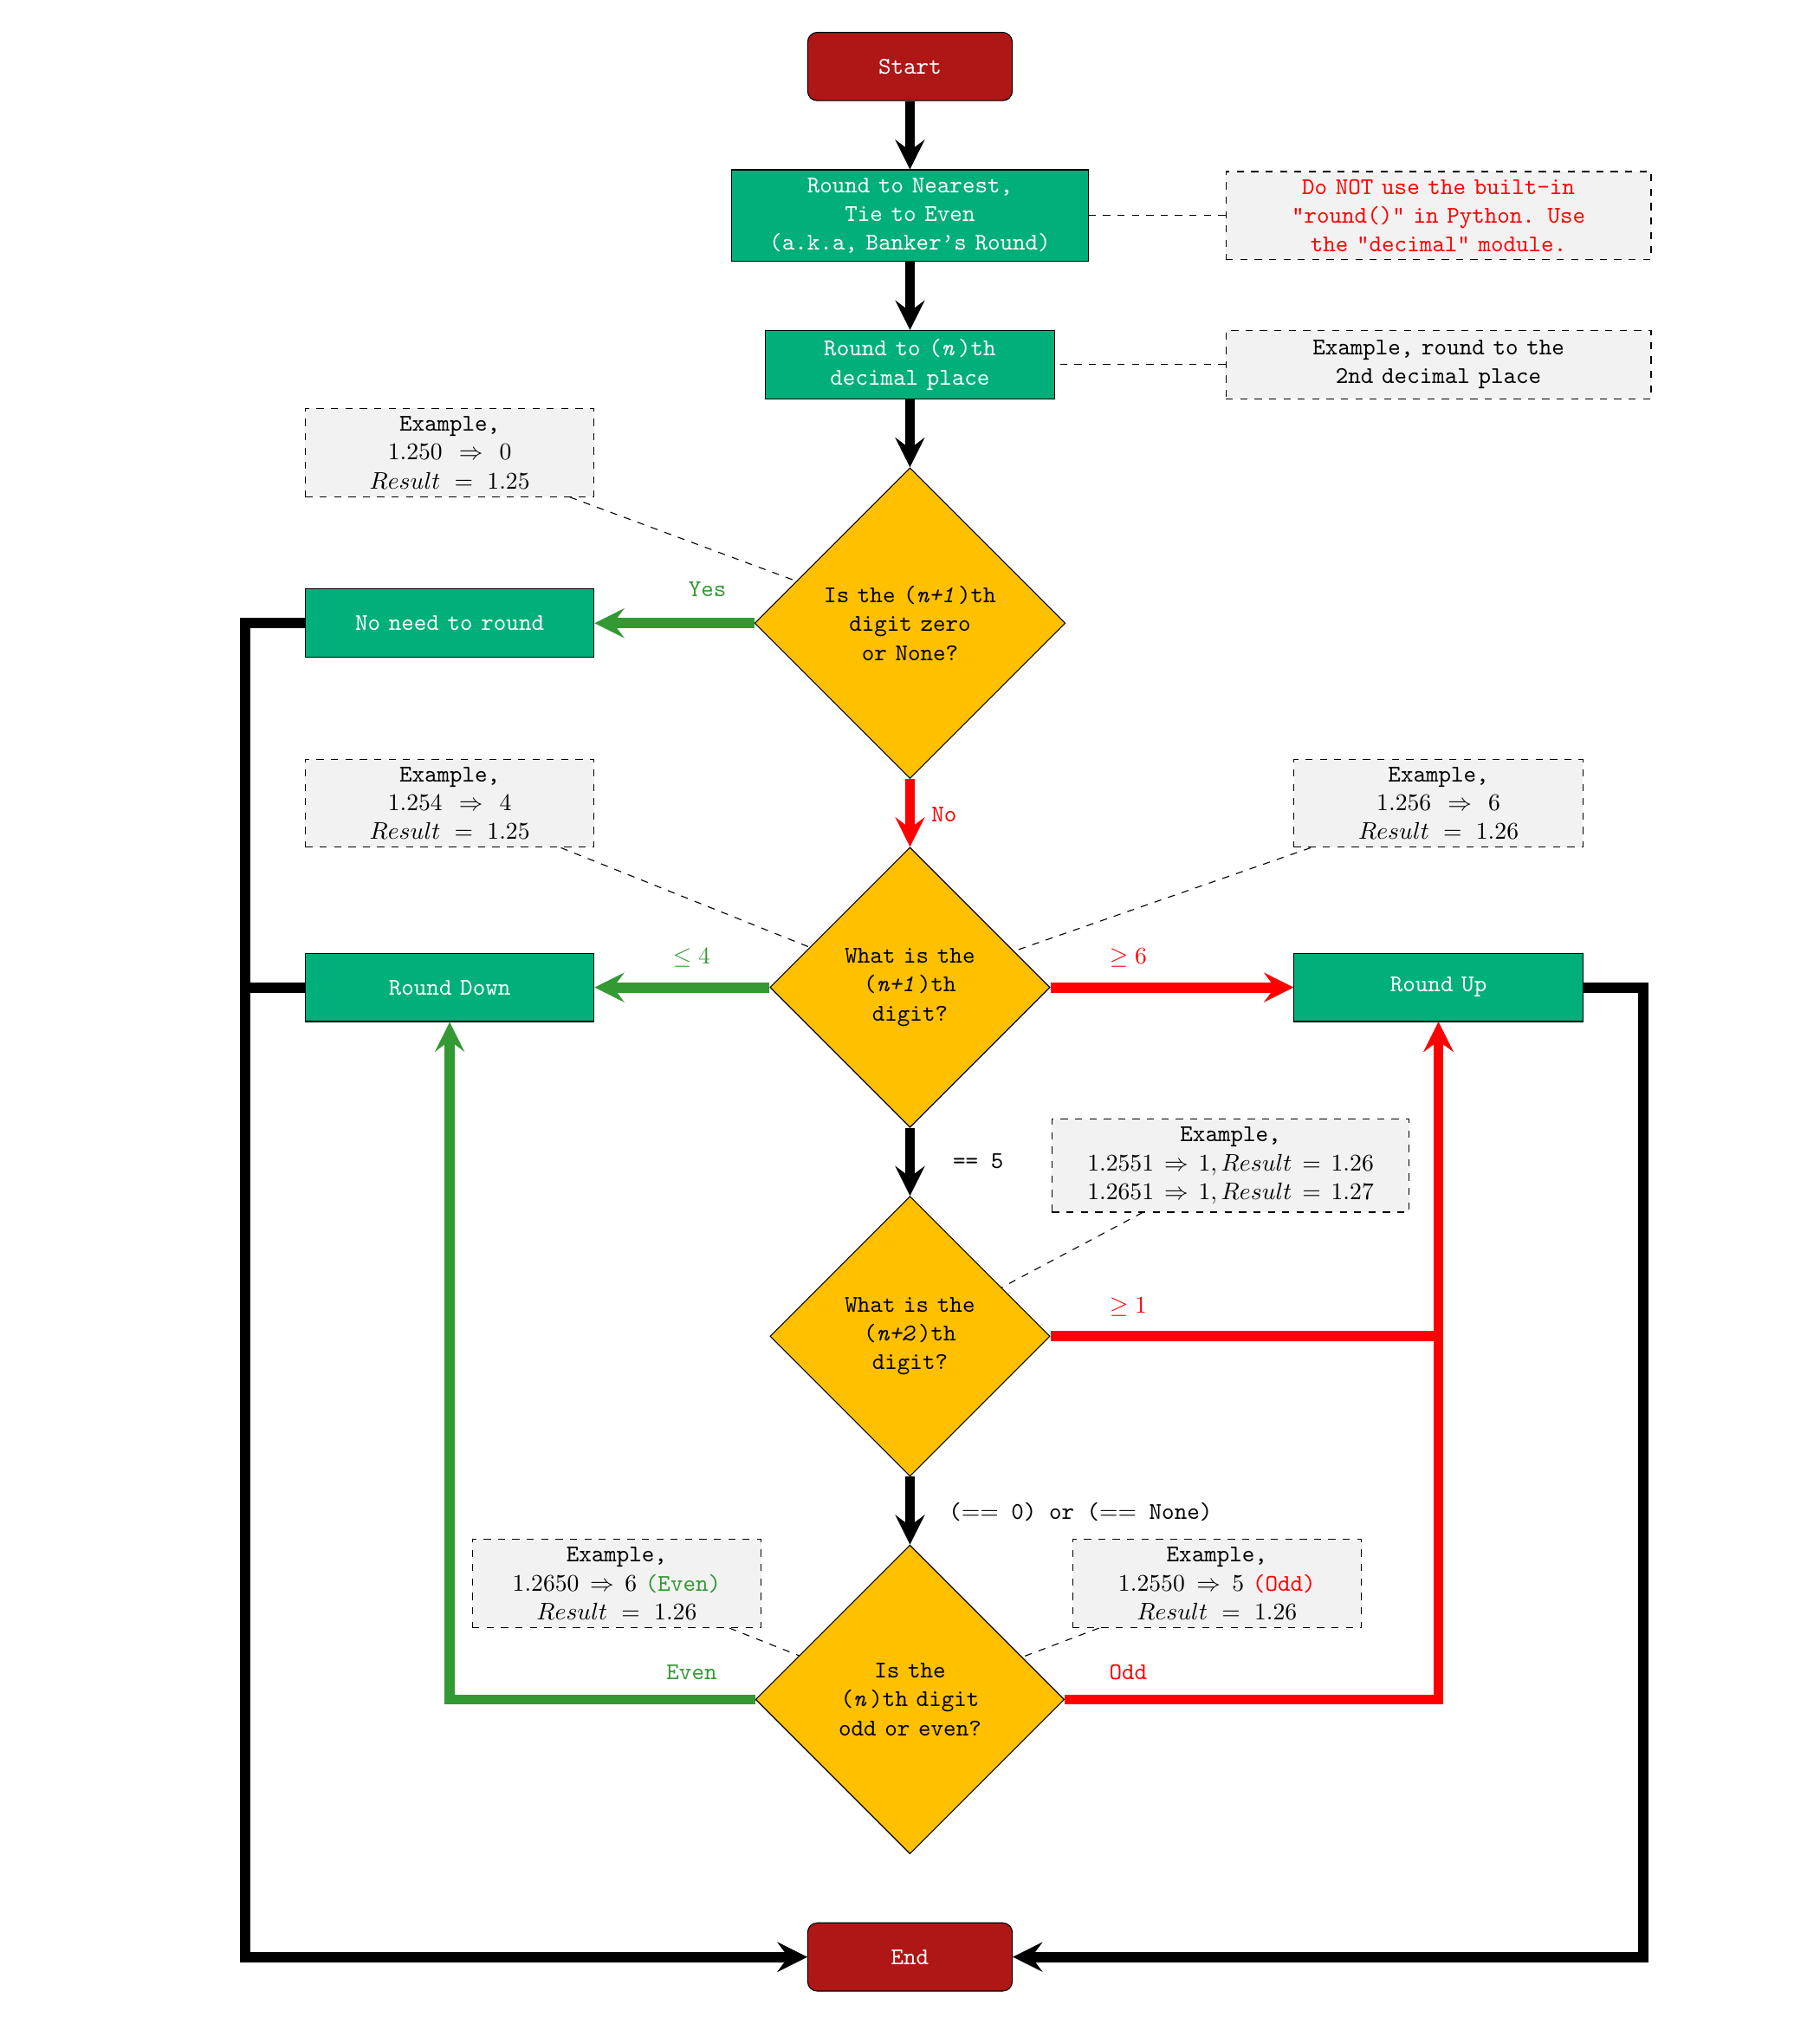
\begin{tikzpicture}[font=\ttfamily\bfseries, baseline=(current bounding box.north), scale=1.0, every node/.style={scale=1}]

		\matrix[column sep=20mm, row sep=10mm]
		{
			% start
			&
			&
			& \node (start)[startstop]{Start};
			& \\

			% round to nearest, tie to even
			&
			&
			& \node (pBankersRound)[process, text width=50mm]{Round to Nearest, Tie to Even \\ (a.k.a, Banker's Round)};
			& \node (cBankersRound)[comment, text width=60mm]{\textcolor{red}{\textbf{Do NOT use the built-in "round()" in Python. Use the "decimal" module.}}};
			& \\

			% round to nearest, tie to even
			&
			&
			& \node (pRound2Nth)[process, text width=40mm]{Round to (\textit{n})th decimal place};
			& \node (expRound2Nth)[comment, text width=60mm]{Example, round to the 2nd decimal place};
			& \\

			&
			& \node (pNoRound)[process, text width=40mm]{No need to round};
			& \node (decNP1Zero)[decision, text width=30mm]{Is the
			(\textit{n+1})th digit zero or None?};
			& \\

			% n+1 th
			&
			& \node (pRoundDown)[process, text width=40mm]{Round Down};
			& \node (decNP1)[decision, text width=25mm]{What is the (\textit{n+1})th digit?};
			& \node (pRoundUp)[process, text width=40mm]{Round Up};
			& \\

			% n+2 th
			&
			&
			& \node (decNP2)[decision, text width=25mm]{What is the (\textit{n+2})th digit?};
			& \\

			% \coordinate[right of=decNP2, xshift=-10mm, yshift=10mm] (expNP2);

			&
			&
			& \node (decNP1_2)[decision, text width=30mm]{Is the (\textit{n})th digit \\ odd or even?};
			& \\

			% end
			&
			&
			& \node (end)[startstop]{End};
			& \\
		};

		\node(expNoRound)[comment, yshift=25mm, text width=40mm] at (pNoRound){Example, \\ $1.250 \Rightarrow 0$ \\ $Result = 1.25$};

		\node(expRoundDownNP1)[comment, yshift=27mm, text width=40mm] at (pRoundDown) {Example, \\ $1.254 \Rightarrow 4$ \\ $Result = 1.25$};

		\node(expRoundUpNP1)[comment, yshift=27mm, text width=40mm] at (pRoundUp) {Example, \\ $1.256 \Rightarrow 6$ \\ $Result = 1.26$};

		\node(expNP2)[comment, xshift=47mm, yshift=25mm, text width=50mm] at (decNP2) {Example, \\ $1.2551 \Rightarrow 1, Result = 1.26$ \\ $1.2651 \Rightarrow 1, Result = 1.27$};

		\node(expNP1_2_odd)[comment, xshift=45mm, yshift=17mm, text width=40mm] at (decNP1_2) {Example, \\ $1.2550 \Rightarrow 5$\ \textcolor{colorNo}{(Odd)} \\ $Result = 1.26$};
		\node(expNP1_2_even)[comment, xshift=-43mm, yshift=17mm, text width=40mm] at (decNP1_2) {Example, \\ $1.2650 \Rightarrow 6$\ \textcolor{colorYes}{(Even)} \\ $Result = 1.26$};


		% lines and arrows
		\draw[arrow](start) -- (pBankersRound);
		\draw[arrow](pBankersRound) -- (pRound2Nth);
		\draw[arrow](pRound2Nth) -- (decNP1Zero);
		\draw[arrow, , color=colorNo](decNP1Zero)node[anchor=north,
		xshift=5mm, yshift=-25mm]{No} -- (decNP1);

		% 拐弯用
		\coordinate[left of=pRoundDown, xshift=-20mm] (dummy1);
		\coordinate[right of=pRoundUp, xshift=20mm] (dummy2);

		\draw[arrow, , color=colorYes](decNP1Zero)node[anchor=east,
		xshift=-25mm, yshift=5mm]{Yes} -- (pNoRound);

		\draw[arrow](pNoRound) -| (dummy1) |- (end);

		\draw[arrow, color=colorYes](decNP1)node[anchor=south, xshift=-32mm, yshift=1mm]{$\leq 4$} -- (pRoundDown);
		\draw[arrow, color=colorNo](decNP1)node[anchor=south, xshift=32mm, yshift=1mm]{$\geq 6$} -- (pRoundUp);
		\draw[arrow](decNP1)node[anchor=north, xshift=10mm, yshift=-22.5mm]{== 5} -- (decNP2);

		\draw[arrow, color=colorNo](decNP2)node[anchor=south, xshift=32mm, yshift=1mm]{$\geq 1$} -| (pRoundUp);
		\draw[arrow](decNP2)node[anchor=north, xshift=25mm, yshift=-22.5mm]{($==$ 0) or ($==$ None) } -- (decNP1_2);

		\draw[arrow, color=colorNo](decNP1_2)node[anchor=south, xshift=32mm, yshift=1mm]{Odd} -| (pRoundUp);
		\draw[arrow, color=colorYes](decNP1_2)node[anchor=south, xshift=-32mm, yshift=1mm]{Even} -| (pRoundDown);

		\draw[arrow](pRoundDown) -- (dummy1) |- (end);
		\draw[arrow](pRoundUp) -- (dummy2) |- (end);

		% dashed line
		\draw[dashed] (cBankersRound) -- (pBankersRound);
		\draw[dashed] (expRound2Nth) -- (pRound2Nth);
		\draw[dashed] (expNoRound) -- (decNP1Zero);
		\draw[dashed] (expRoundDownNP1) -- (decNP1);
		\draw[dashed] (expRoundUpNP1) -- (decNP1);
		\draw[dashed] (expNP2) -- (decNP2);
		\draw[dashed] (expNP1_2_odd) -- (decNP1_2);
		\draw[dashed] (expNP1_2_even) -- (decNP1_2);

	\end{tikzpicture}

	\begin{tikzpicture}[baseline=(current bounding box.north), scale=1.0, every node/.style={scale=1}]

		\matrix[column sep=20mm, row sep=10mm]
		{
			% start
			&
			&
			& \node (start)[startstop]{开始};
			& \\

			% round to nearest, tie to even
			&
			&
			& \node (pBankersRound)[process, text width=50mm]{四舍六入五留双 \\ (亦称作“银行家数值修约”)};
			& \node (cBankersRound)[comment, text width=60mm]{\textcolor{red}{不要使用Python自带的“round()”函数。应使用“decimal”模块。}};
			& \\

			% round to nearest, tie to even
			&
			&
			& \node (pRound2Nth)[process, text width=40mm]{保留$n$位数字};
			& \node (expRound2Nth)[comment, text width=60mm]{例:保留两位数字};
			& \\

			&
			&
			& \node (pTims10N)[process, text width=40mm]{将输入数字乘以$10^n$};
			& \\

			&
			& \node (pNoRound)[process, text width=40mm]{不需要修约};
			& \node (decNP1Zero)[decision, text width=25mm]{新数字是否为整数?};
			& \\

			&
			& \node (pRoundDown)[process, text width=40mm]{舍位};
			& \node (decNP1)[decision, text width=30mm]{新数字的小数部分是?};
			& \node (pRoundUp)[process, text width=40mm]{进位};
			& \\

			&
			&
			& \node (decNP2)[decision, text width=30mm]{新数字的整数部分是否为偶?};
			& \\

			% end
			&
			&
			& \node (end)[startstop]{结束};
			& \\
		};

		\node(expNoRound)[comment, yshift=25mm, text width=40mm] at (pNoRound){例: $1.250 \Rightarrow 125.0$ \\ 结果 $= 1.25$};

		\node(expNP1Big)[comment, xshift=0mm, yshift=25mm, text width=40mm] at (pRoundUp) {例: \\ $1.2551 \Rightarrow 125.51$ \\ $0.51 > 0.5$ \\ 结果 $= 1.26$};
		\node(expNP1Small)[comment, xshift=0mm, yshift=25mm, text width=40mm] at (pRoundDown) {例: \\ $1.2541 \Rightarrow 125.41$ \\ $0.41 < 0.5$ \\ 结果 $= 1.25$};

		\node(expNP1_2_odd)[comment, xshift=45mm, yshift=25mm, text width=40mm] at (decNP2) {例: \\ $1.2550 \Rightarrow 125.50$ \\ $125$为\textcolor{red}{奇} \\ 结果 $= 1.26$};
		\node(expNP1_2_even)[comment, xshift=-43mm, yshift=25mm, text width=40mm] at (decNP2) {例: \\ $1.2450 \Rightarrow 124.50$ \\ $124$为\textcolor{colorYes}{偶} \\ 结果 $= 1.24$};


		% 拐弯用
		\coordinate[left of=pRoundDown, xshift=-20mm] (dummy1);
		\coordinate[right of=pRoundUp, xshift=20mm] (dummy2);

		% lines and arrows
		\draw[arrow](start) -- (pBankersRound);
		\draw[arrow](pBankersRound) -- (pRound2Nth);
		\draw[arrow](pRound2Nth) -- (pTims10N);
		\draw[arrow](pTims10N) -- (decNP1Zero);

		\draw[arrow, color=colorYes](decNP1Zero)node[anchor=south, xshift=-25mm, yshift=1mm]{是} -- (pNoRound);
		\draw[arrow, color=colorNo](decNP1Zero)node[anchor=north, xshift=5mm, yshift=-20mm]{否} -- (decNP1);

		\draw[arrow](pNoRound) -| (dummy1) |- (end);

		\draw[arrow, color=colorYes](decNP1)node[anchor=south, xshift=-32mm, yshift=1mm]{小于0.5} -- (pRoundDown);
		\draw[arrow, color=colorNo](decNP1)node[anchor=south, xshift=34mm, yshift=1mm]{大于0.5} -- (pRoundUp);
		\draw[arrow](decNP1)node[anchor=north, xshift=12mm, yshift=-23mm]{等于0.5} -- (decNP2);

		\draw[arrow, color=colorNo](decNP2)node[anchor=south, xshift=40mm, yshift=1mm]{否(奇)} -| (pRoundUp);
		\draw[arrow, color=colorYes](decNP2)node[anchor=south, xshift=-40mm, yshift=1mm]{是(偶)} -| (pRoundDown);

		\draw[arrow](pRoundDown) -- (dummy1) |- (end);
		\draw[arrow](pRoundUp) -- (dummy2) |- (end);

		% dashed line
		\draw[dashed] (cBankersRound) -- (pBankersRound);
		\draw[dashed] (expRound2Nth) -- (pRound2Nth);
		\draw[dashed] (expNoRound) -- (decNP1Zero);
		\draw[dashed] (expNP1Big) -- (decNP1);
		\draw[dashed] (expNP1Small) -- (decNP1);
		\draw[dashed] (expNP1_2_odd) -- (decNP2);
		\draw[dashed] (expNP1_2_even) -- (decNP2);

	\end{tikzpicture}
	\begin{tikzpicture}[baseline=(current bounding box.north), scale=1.0, every node/.style={scale=1}]

		\matrix[column sep=20mm, row sep=10mm]
		{
			% start
			&
			&
			& \node (start)[startstop]{開始};
			& \\

			% round to nearest, tie to even
			&
			&
			& \node (pBankersRound)[process, text width=50mm]{四捨六入五留雙 \\ (亦稱作“銀行家數值修約”)};
			& \node (cBankersRound)[comment, text width=60mm]{\textcolor{red}{不要使用Python自帶的“round()”函數。應使用“decimal”模塊。}};
			& \\

			% round to nearest, tie to even
			&
			&
			& \node (pRound2Nth)[process, text width=40mm]{保留$n$位數字};
			& \node (expRound2Nth)[comment, text width=60mm]{例:保留兩位數字};
			& \\

			&
			&
			& \node (pTims10N)[process, text width=40mm]{將輸入數字乘以$10^n$};
			& \\

			&
			& \node (pNoRound)[process, text width=40mm]{不需要修約};
			& \node (decNP1Zero)[decision, text width=25mm]{新數字是否爲整數?};
			& \\

			&
			& \node (pRoundDown)[process, text width=40mm]{舍位};
			& \node (decNP1)[decision, text width=30mm]{新數字的小數部分是?};
			& \node (pRoundUp)[process, text width=40mm]{進位};
			& \\

			&
			&
			& \node (decNP2)[decision, text width=30mm]{新數字的整數部分是否爲偶?};
			& \\

			% end
			&
			&
			& \node (end)[startstop]{結束};
			& \\
		};

		\node(expNoRound)[comment, yshift=25mm, text width=40mm] at (pNoRound){例: $1.250 \Rightarrow 125.0$ \\ 結果 $= 1.25$};

		\node(expNP1Big)[comment, xshift=0mm, yshift=25mm, text width=40mm] at (pRoundUp) {例: \\ $1.2551 \Rightarrow 125.51$ \\ $0.51 > 0.5$ \\ 結果 $= 1.26$};
		\node(expNP1Small)[comment, xshift=0mm, yshift=25mm, text width=40mm] at (pRoundDown) {例: \\ $1.2541 \Rightarrow 125.41$ \\ $0.41 < 0.5$ \\ 結果 $= 1.25$};

		\node(expNP1_2_odd)[comment, xshift=45mm, yshift=25mm, text width=40mm] at (decNP2) {例: \\ $1.2550 \Rightarrow 125.50$ \\ $125$爲\textcolor{red}{奇} \\ 結果 $= 1.26$};
		\node(expNP1_2_even)[comment, xshift=-43mm, yshift=25mm, text width=40mm] at (decNP2) {例: \\ $1.2450 \Rightarrow 124.50$ \\ $124$爲\textcolor{colorYes}{偶} \\ 結果 $= 1.24$};


		% 拐弯用
		\coordinate[left of=pRoundDown, xshift=-20mm] (dummy1);
		\coordinate[right of=pRoundUp, xshift=20mm] (dummy2);

		% lines and arrows
		\draw[arrow](start) -- (pBankersRound);
		\draw[arrow](pBankersRound) -- (pRound2Nth);
		\draw[arrow](pRound2Nth) -- (pTims10N);
		\draw[arrow](pTims10N) -- (decNP1Zero);

		\draw[arrow, color=colorYes](decNP1Zero)node[anchor=south, xshift=-25mm, yshift=1mm]{是} -- (pNoRound);
		\draw[arrow, color=colorNo](decNP1Zero)node[anchor=north, xshift=5mm, yshift=-20mm]{否} -- (decNP1);

		\draw[arrow](pNoRound) -| (dummy1) |- (end);

		\draw[arrow, color=colorYes](decNP1)node[anchor=south, xshift=-32mm, yshift=1mm]{小於0.5} -- (pRoundDown);
		\draw[arrow, color=colorNo](decNP1)node[anchor=south, xshift=34mm, yshift=1mm]{大於0.5} -- (pRoundUp);
		\draw[arrow](decNP1)node[anchor=north, xshift=12mm, yshift=-23mm]{等於0.5} -- (decNP2);

		\draw[arrow, color=colorNo](decNP2)node[anchor=south, xshift=40mm, yshift=1mm]{否(奇)} -| (pRoundUp);
		\draw[arrow, color=colorYes](decNP2)node[anchor=south, xshift=-40mm, yshift=1mm]{是(偶)} -| (pRoundDown);

		\draw[arrow](pRoundDown) -- (dummy1) |- (end);
		\draw[arrow](pRoundUp) -- (dummy2) |- (end);

		% dashed line
		\draw[dashed] (cBankersRound) -- (pBankersRound);
		\draw[dashed] (expRound2Nth) -- (pRound2Nth);
		\draw[dashed] (expNoRound) -- (decNP1Zero);
		\draw[dashed] (expNP1Big) -- (decNP1);
		\draw[dashed] (expNP1Small) -- (decNP1);
		\draw[dashed] (expNP1_2_odd) -- (decNP2);
		\draw[dashed] (expNP1_2_even) -- (decNP2);

	\end{tikzpicture}
	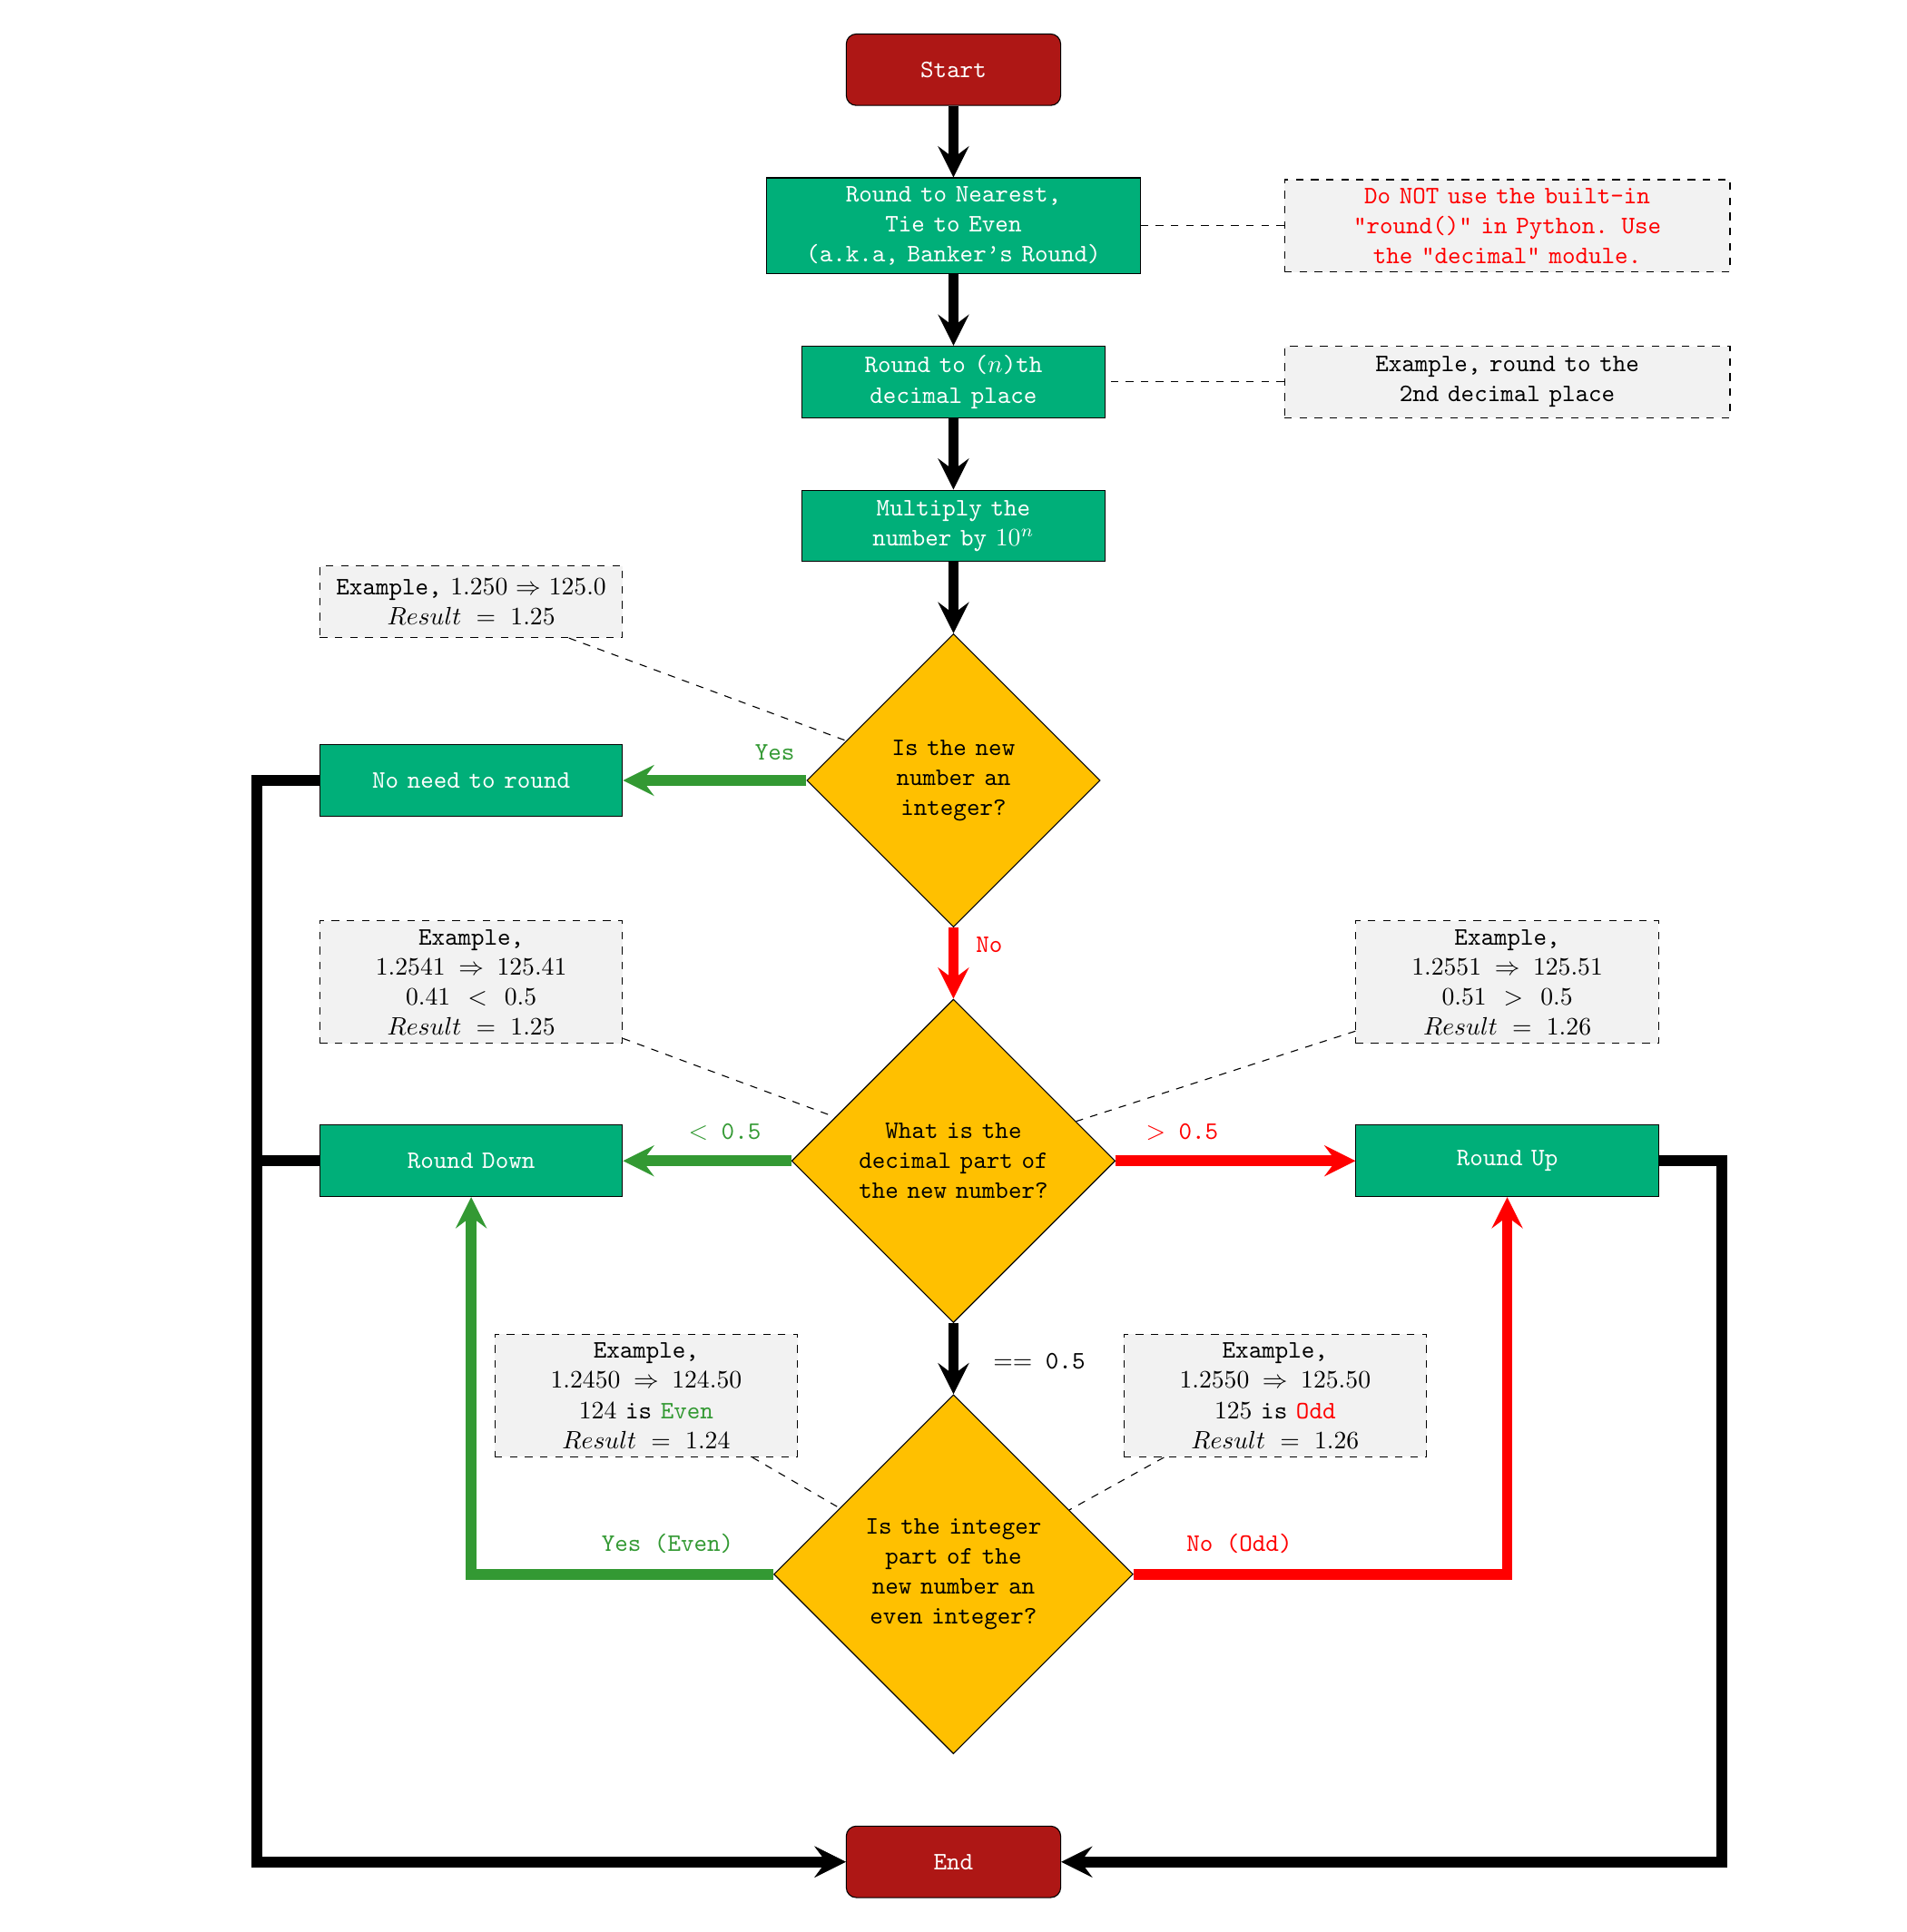
\begin{tikzpicture}[font=\ttfamily\bfseries, baseline=(current bounding box.north), scale=1.0, every node/.style={scale=1}]

		\matrix[column sep=20mm, row sep=10mm]
		{
			% start
			&
			&
			& \node (start)[startstop]{Start};
			& \\

			% round to nearest, tie to even
			&
			&
			& \node (pBankersRound)[process, text width=50mm]{Round to Nearest, Tie to Even \\ (a.k.a, Banker's Round)};
			& \node (cBankersRound)[comment, text width=60mm]{\textcolor{red}{\textbf{Do NOT use the built-in "round()" in Python. Use the "decimal" module.}}};
			& \\

			% round to nearest, tie to even
			&
			&
			& \node (pRound2Nth)[process, text width=40mm]{Round to ({$n$})th decimal place};
			& \node (expRound2Nth)[comment, text width=60mm]{Example, round to the 2nd decimal place};
			& \\

			&
			&
			& \node (pTims10N)[process, text width=40mm]{Multiply the number by $10^n$};
			& \\

			&
			& \node (pNoRound)[process, text width=40mm]{No need to round};
			& \node (decNP1Zero)[decision, text width=25mm]{Is the new number an integer?};
			& \\

			&
			& \node (pRoundDown)[process, text width=40mm]{Round Down};
			& \node (decNP1)[decision, text width=30mm]{What is the decimal part of the new number?};
			& \node (pRoundUp)[process, text width=40mm]{Round Up};
			& \\

			&
			&
			& \node (decNP2)[decision, text width=30mm]{Is the integer part of the new number an even integer?};
			& \\

			% end
			&
			&
			& \node (end)[startstop]{End};
			& \\
		};

		\node(expNoRound)[comment, yshift=25mm, text width=40mm] at (pNoRound){Example, $1.250 \Rightarrow 125.0$ \\ $Result = 1.25$};

		\node(expNP1Big)[comment, xshift=0mm, yshift=25mm, text width=40mm] at (pRoundUp) {Example, \\ $1.2551 \Rightarrow 125.51$ \\ $0.51 > 0.5$ \\ $Result = 1.26$};
		\node(expNP1Small)[comment, xshift=0mm, yshift=25mm, text width=40mm] at (pRoundDown) {Example, \\ $1.2541 \Rightarrow 125.41$ \\ $0.41 < 0.5$ \\ $Result = 1.25$};

		\node(expNP1_2_odd)[comment, xshift=45mm, yshift=25mm, text width=40mm] at (decNP2) {Example, \\ $1.2550 \Rightarrow 125.50$ \\ $125$ is \textcolor{red}{Odd} \\ $Result = 1.26$};
		\node(expNP1_2_even)[comment, xshift=-43mm, yshift=25mm, text width=40mm] at (decNP2) {Example, \\ $1.2450 \Rightarrow 124.50$ \\ $124$ is \textcolor{colorYes}{Even} \\ $Result = 1.24$};


		% 拐弯用
		\coordinate[left of=pRoundDown, xshift=-20mm] (dummy1);
		\coordinate[right of=pRoundUp, xshift=20mm] (dummy2);

		% lines and arrows
		\draw[arrow](start) -- (pBankersRound);
		\draw[arrow](pBankersRound) -- (pRound2Nth);
		\draw[arrow](pRound2Nth) -- (pTims10N);
		\draw[arrow](pTims10N) -- (decNP1Zero);

		\draw[arrow, color=colorYes](decNP1Zero)node[anchor=south, xshift=-25mm, yshift=1mm]{Yes} -- (pNoRound);
		\draw[arrow, color=colorNo](decNP1Zero)node[anchor=north, xshift=5mm, yshift=-20mm]{No} -- (decNP1);

		\draw[arrow](pNoRound) -| (dummy1) |- (end);

		\draw[arrow, color=colorYes](decNP1)node[anchor=south, xshift=-32mm, yshift=1mm]{$<$ 0.5} -- (pRoundDown);
		\draw[arrow, color=colorNo](decNP1)node[anchor=south, xshift=32mm, yshift=1mm]{$>$ 0.5} -- (pRoundUp);
		\draw[arrow](decNP1)node[anchor=north, xshift=12mm, yshift=-25mm]{$==$ 0.5} -- (decNP2);

		\draw[arrow, color=colorNo](decNP2)node[anchor=south, xshift=40mm, yshift=1mm]{No (Odd)} -| (pRoundUp);
		\draw[arrow, color=colorYes](decNP2)node[anchor=south, xshift=-40mm, yshift=1mm]{Yes (Even)} -| (pRoundDown);

		\draw[arrow](pRoundDown) -- (dummy1) |- (end);
		\draw[arrow](pRoundUp) -- (dummy2) |- (end);

		% dashed line
		\draw[dashed] (cBankersRound) -- (pBankersRound);
		\draw[dashed] (expRound2Nth) -- (pRound2Nth);
		\draw[dashed] (expNoRound) -- (decNP1Zero);
		\draw[dashed] (expNP1Big) -- (decNP1);
		\draw[dashed] (expNP1Small) -- (decNP1);
		\draw[dashed] (expNP1_2_odd) -- (decNP2);
		\draw[dashed] (expNP1_2_even) -- (decNP2);

	\end{tikzpicture}

\end{document}